\documentclass[12pt, twoside, a4paper]{article}
\usepackage[left = 20mm, top = 20mm]{geometry}
\usepackage{amsmath,amsthm,amssymb,amsfonts}
\usepackage[makeroom]{cancel}
\newcommand{\Gen}{\mathcal{L}}
\usepackage[parfill]{parskip}
\usepackage{graphicx}
\usepackage{enumerate}

\begin{document}

\section{Kingman's Coalescent}
\begin{enumerate}[a)]
\item
The only possible transition at time $t$ is to go from $N_t$ to $N_t - 1$, so the rate as a function of the number of particles $k$ is
\[g(k, k-1) = 
\begin{cases}
	{k \choose 2} & \text{for } 1 < k \le L\\
	0 & \text{otherwise.}
\end{cases}
\]
The generator is given by 
\begin{align*}
(\Gen f)(k) &= \sum_{\substack{j \in S \\ j \neq k}} g(k, j)[f(j) - f(k)]\\
&= g(k, k-1)[f(k-1)-f(k)]\\
&= {k \choose 2} \bigg[f(k-1) - f(k) \bigg]\text{,}
\end{align*}
and the master equation
\begin{align*}
\frac{d}{dt}\pi \textsubscript{t} (k) &= \sum_{j \neq k} \pi \textsubscript{t} (j) g(j, k) - \sum_{j \neq k} \pi \textsubscript{t} (k) g(k, j)\\
&= \pi \textsubscript{t} (k+1) g(k+1, k) \\
&= \pi \textsubscript{t} (k + 1) {k+1 \choose 2} - \pi \textsubscript{t} (k) {k \choose 2} \text{.}
\end{align*}
The process has one absorbing state at $k = 1$ since it needs two particle to coalesce, so once it reaches the one particle state nothing will happen. This also describes the stationary distribution given by $(1, 0, 0, \dots)$, and since the process converges to this stationary distribution from any starting state, the process is ergodic. 

\item
Since the expected staying time in state $k$ is $1/g(k, k-1)$, the total time to go from $k = L$ to $k = 1$ is the sum of all the expected times, i.e.,
\begin{align*}
\mathbb{E}(T) 
&= \sum_{k = 2}^{L} \bigg[{k \choose 2} \bigg] ^{-1}
= \sum_{k=2}^{L} \frac{2! \, (k-2)!}{k!}\\
&= 2 \sum_{k = 2}^{L} \frac{1}{k(k-1)}
= 2 \sum_{k = 2}^{L} \bigg( \frac{1}{k-1} - \frac{1}{k} \bigg)\\
&= 2 \bigg[ \bigg( \frac{1}{1} - \bcancel{\frac{1}{2}} \bigg)
		   +\bigg( \bcancel{\frac{1}{2}} -  \bcancel{\frac{1}{3}} \bigg)
		   + \dots
		   +\bigg(  \bcancel{\frac{1}{1-L}} - \frac{1}{L} \bigg) \bigg]\\
&= 2 \bigg( 1 - \frac{1}{L} \bigg) 
\end{align*}
\qed

\item
The generator for the rescaled process $N_t / L$ is given by 
\[
(\Gen f)(x) = {xL \choose 2} \bigg[ f \bigg(x - \frac{1}{L} \bigg) - f(x) \bigg] \text{,}
\]
where $x = k/L$. Using Taylor expansion for $f(x-1/L)$ around $f(x)$ gives
\begin{align*}
f \bigg(x - \frac{1}{L} \bigg) &= f(x) - \frac{1}{L}f'(x) + \frac{1}{2L^2}f''(x) + \dots \text{, so }\\
(\Gen f)(x) &= {xL \choose 2} \bigg[ \frac{1}{2L^2}f''(x) - \frac{1}{L}f'(x) \bigg]
\end{align*}
Slowing the process down just applies a factor of $1/L$ to the rates. The generator for $X_t^L= \frac{1}{L} N \textsubscript{t/L}$ is then 
\begin{align*}
(\Gen f)(x) 
&= \frac{1}{L} \cdot \frac{(Lx)!}{2! \, (Lx-2)!} \bigg[ \frac{1}{2L^2}f''(x) - \frac{1}{L}f'(x) \bigg]\\
&= \frac{(\bcancel{L}x)(Lx-1)}{2\bcancel{L}} \bigg[ \frac{1}{2L^2}f''(x) - \frac{1}{L}f'(x) \bigg]\\
&= \frac{1}{2} \bigg[ \bcancel{\frac{x^2}{2L}f''(x)} - x^2 f'(x) - \bcancel{\frac{x^2}{2L}f''(x)} + \cancelto{0}{\frac{x}{L}f'(x)} \bigg]\\
&= - \frac{x^2}{2} f'(x) \text{ as } L \to \infty \text{.}
\end{align*}
Since the process $X_t^L$ starts at $x = L/L = 1$ and always terminates at $x = 1/L \neq 0$, the state space $(0, 1]$ is open at $0$ and  $X \textsubscript{0} = 1$.

We see that this corresponds to the generator of a diffusion process with only the drift term but no diffusion which specifies the randomness. Therefore the process is deterministic because there is no randomness. 

In order to compute $X_t$ explicitly, we start with an SDE with no diffusion term and integrate both sides
\begin{align*}
dX_t &= a(X_t, t) dt \\
\int_0^t dX_s &= \int_0^t \frac{-X_s^2}{2} ds \\
\int_0^t X_s^{-2} dX_s &= - \int_0^t \frac{1}{2} ds \\ 
X_s^{-1} \, \Big| _0^t &= \frac{1}{2} s \, \Big| _0^t
\end{align*}

By evaluating this integral and substituting $X_0 = 1$, we arrive at the explicit solution
\[
X_t = \frac{2}{2+t} \, \text{.}
\]

This is compatible with the result from part b) because the results are for differently scaled processes. i.e., $2/(2+t)$ describes the path of $X_t^L$ which we have defined to be $\frac{1}{L} N_{t/L} \, $, whereas the mean time to absorption calculated in part b) is for the unscaled process $N_t$. By applying the appropriate scaling, we have 
\[
N_t = L \cdot \frac{2}{2+tL} \, \text{,}
\]
from which we can deduce that 
\[N_t = 1 \implies t = \mathbb{E} (T) = 2 \bigg(1 - \frac{1}{L} \bigg) \, \text{,}
\]
which is in line with our results from part b).

\item
\text{}\\
\hspace*{-2cm}
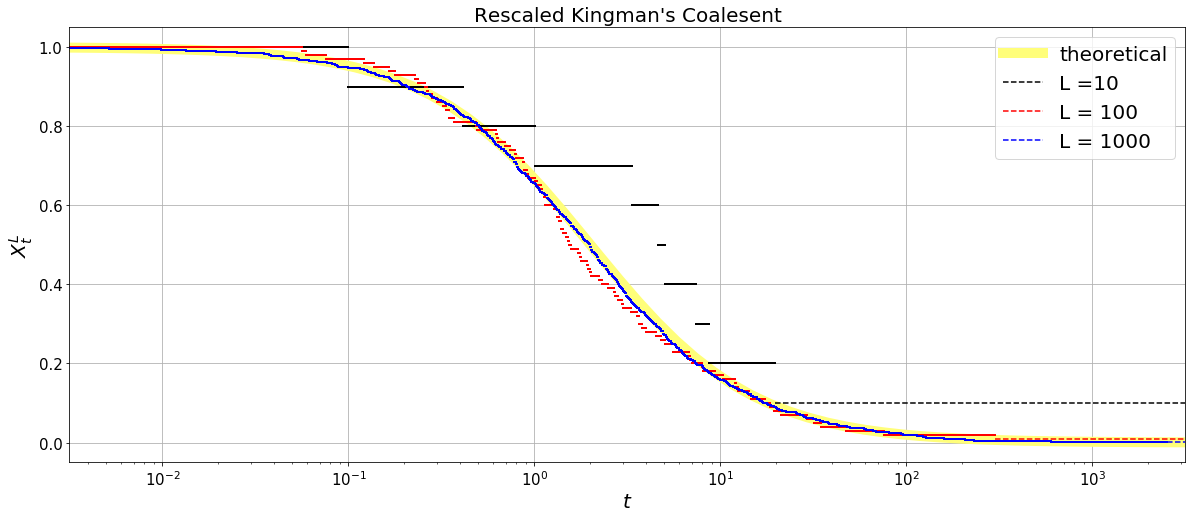
\includegraphics[width=19cm]{Kingman}
\end{enumerate}

\section{Orstein-Uhlenbeck process}
\begin{enumerate}
\item [a+b)]
Let $f(X_t) = X_t$, then $f'(X_t) = 1$ and $f''(X_t) = 0$, and using the evolution equation, 
\[
\frac{d}{dt} \mathbb{E} [X_t] = \mathbb{E} [ - \alpha X_t ] = - \alpha \mathbb{E} [X_t] \text{,}
\]
so
\[
\frac{d}{dt} \mathbb{E} [X_t] + \alpha \mathbb{E} [X_t] = 0
\]
is the required ODE. 
Solving this gives the general solution $m(t) := \mathbb{E} [X_t] = Ae^{- \alpha t}$, where $A$ is an arbitrary constant. We can then substitute in $m(0) = x_0$ to obtain 
\[
m(t) = x_0 e^{- \alpha t} \text{.}
\]
Similarly, let $f(X_t) = X_t^2$, then $f'(X_t) = 2X_t$ and $f''(X_t) = 2$, and 
\[
\frac{d}{dt} \mathbb{E} [X_t^2] = \mathbb{E} [ - \alpha X_t \cdot 2X_t + \frac{1}{2} \sigma ^2 \cdot 2 ] = - \alpha \mathbb{E} [X_t^2] + \sigma ^2 \text{,}
\]
so
\[
\frac{d}{dt} \mathbb{E} [X_t^2] + 2 \alpha \mathbb{E} [X_t^2] = \sigma ^2 \text{,}
\]
which can be solved to give $\mathbb{E} [X_t^2] = \sigma ^2/2 \alpha + Be^{-2 \alpha t}$, where $B$ is an arbitrary constant. Therefore, 
\begin{align*}
v(t) = \mathbb{E} [X_t^2] - (\mathbb{E} [X_t])^2 &= \frac{\sigma ^2}{2 \alpha} + Be^{-2 \alpha t} - (Ae^{- \alpha t})^2\\
&= \frac{\sigma ^2}{2 \alpha} + Ce^{-2 \alpha t} \text{.}
\end{align*}
But we know that $v(0) = 0$ because the process is deterministic at $t = 0$, so we can use this fact to obtain 
\[
v(t) = \frac{\sigma ^2}{2 \alpha} \big( 1 - e^{-2 \alpha t} \big) \text{.}
\]
Therefore the distribution of $X_t$ is $X_t \sim \mathcal{N} \big( m(t), v(t) \big)$.

As $t \to \infty$, $m(t) \to 0$ and $v(t) \to \tfrac{\sigma ^2}{2 \alpha}$, so the stationary distribution of the process is $X_t \sim \mathcal{N} \big( 0, \tfrac{\sigma ^2}{2 \alpha} \big)$.

\item[c)]
\text{}\\
\hspace*{-2cm}
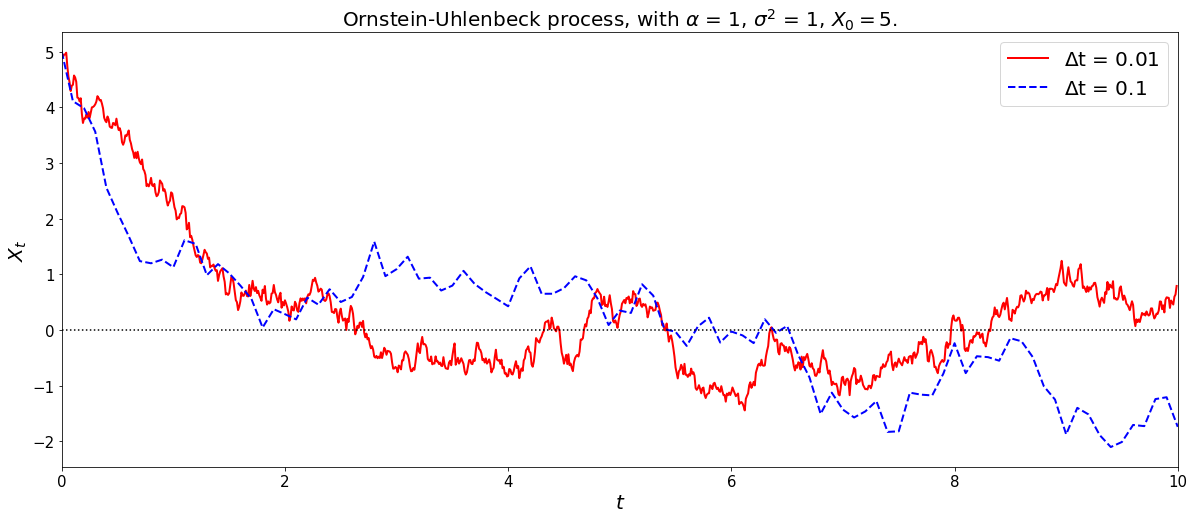
\includegraphics[width = 190mm]{O-U}

\end{enumerate}

\section{Moran model and Wright-Fisher diffusion}
\begin{enumerate}[a)]
\item
The state space of $(X_t : t \geq 0)$ is $\{ (x_1, x_2, \dots, x_L) : x_i \in \{ 1, 2, \dots, L\}\}$. The process is not reducible since once a type has been completely killed off, the process can no longer return to a state where one of the individuals is of that type.

The stationary distributions are $\{(x, x, \dots, x) : x \in \{1, 2, \dots, L\}\}$ because the process is only stationary once only a single type survives. 

\item
$(N_t : t \geq 0)$ is a Markov process and its state space is $\{0, 1, \dots, L\}$. 

The rates of this process for $x \neq 0 \text{ or } L$ is 
\begin{align*}
\begin{cases}
g(x, x+1) &= x \cdot \frac{L-x}{L-1}\\
g(x, x-1) &= (L-x) \cdot \frac{x}{L-1}
\end{cases}
\end{align*}
The reasoning is that in order to gain an individual, one of the $x$ current individuals must impose its type on someone of a different type. Since it does so randomly, the probability of killing someone of a different type is $\frac{L-x}{L-1}$. We also get $g(x, x-1)$ by applying similar logic. 

The generator is 
\[
(\Gen f) (x) = \frac{x(L-x)}{L-1} [f(x+1) - 2f(x) + f(x-1)] \text{.}
\]

The process is, once again, not irreducible since $x = 0$ and $x = L$ are absorbing states. This also means that there exist infinitely many stationary distributions of the form 
\[
(\alpha, 0, \dots, 1- \alpha) \text{ , } \alpha \in [0, 1] \text{.}
\]

The limiting distribution as $t \to \infty$ is 
\[
\bigg( \frac{L-1}{L}, 0, \dots, 0, \frac{1}{L} \bigg)
\]
since the probability of any one individual dominating is exactly the same due to symmetry, and there was only one individual of type $k$ at $t = 0$. 

\item
By setting $f(N_t) = N_t$ and using the evolution equation, we obtain 
\[
\frac{d}{dt} \mathbb{E} [N_t] = \mathbb{E} \bigg[ \frac{N_t (L-N_t)}{L-1} \bigg( (N_t+1) - 2(N_t) + (N_t-1) \bigg) \bigg] = 0 \text{,}
\]
which means that $N_t$ is constant in time. Given that $N_0 = n$, we may deduce that $m_1(t) \equiv n$. 

Similarly, by setting $f(N_t) = N_t^2$, 
\begin{align*}
\frac{d}{dt} \mathbb{E} [N_t^2] 
&= \mathbb{E} \bigg[ \frac{N_t (L-N_t)}{L-1} \bigg( (N_t^2 + 2 N_t +1) - 2(N_t^2) + (N_t^2 - 2 N_t +1) \bigg) \bigg] \\
&= \mathbb{E} \bigg[ \frac{2 N_t (L - N_t)}{L-1} \bigg]\\
&= \frac{2L}{L-1} \mathbb{E} [N_t] - \frac{2}{L-1} \mathbb{E} [N_t^2]
\end{align*}

i.e., 
\[
\frac{d}{dt} \mathbb{E} [N_t^2] + \frac{2}{L-1} \mathbb{E} [N_t^2] = \frac{2Ln}{L-1} \text{.}
\]

Solving this gives
\[
m_2(t) = \mathbb{E} [N_t^2] = Ln + Ae^{\frac{2t}{1-L}}
\]

In the scaling limit $t \to \infty$, the exponential term vanishes so we just have $m_2(t) \to Ln \,$. 

As shown in part b), the probability of any one individual dominating the population is $\tfrac{1}{L}$, and this is independent of the individual's type. We may then deduce that the probability of a given type, which starts with $n$ individuals, dominating - i.e., being absorbed in $N = L$ - is equal to $\tfrac{n}{L}$. Since we are considering the scaling limit $t \to \infty$, the process must be in one of the absorbing states, so the probability of being absorbed at 0 is $1-\tfrac{n}{L}$.

Using $m_1(t)$, $m_2(t)$, and the fact that the process is deterministic at $t=0$, we can obtain 
\[
v(t) = (Ln-n^2)(1- e^{\frac{-2t}{L-1}}) \text{.}
\]
It follows that when $L$ is large, the variance scales linearly with $L$ so the absorption time is also linear in $L$. 

\item
Rescaling the generator gives
\[
(\Gen f) (x) = L^\alpha \cdot \frac{xL(L-xL)}{L-1} \bigg[ f \big( x+\tfrac{1}{L} \big) - 2f(x) + f \big( x-\tfrac{1}{L} \big) \bigg] \text{.}
\]
By using Taylor expansion around $x$ for terms up to second order, we have 
\begin{align*}
(\Gen f) (x) &= L^\alpha \cdot \frac{\bcancel{L^2}}{L-1} \cdot x(1-x) \cdot \frac{1}{\bcancel{L^2}} f''(x)\\
&= \frac{L^\alpha}{L-1} \cdot x(1-x) f''(x) \text{.}
\end{align*}
We can see that the only $\alpha$ for which $M_t^L$ has a non-trivial scaling limit is when $\alpha = 1$, thus we have the generator for $(M_t : t \geq 0)$ is 
\[
(\Gen f) (x) = x(1-x) f''(x) \text{,}
\]
which essentially describes a diffusion process with no drift term. This makes sense as the process is essentially completely random. Substituting $a(x, t) = 0$ and $\tfrac{\sigma ^2}{2} (x, t) = x(1-x)$ into the Fokker-Planck equation gives
\[
\frac{\partial}{\partial t} p_t(x, y) = \frac{\partial ^2}{\partial y^2} \big( y(1-y)p_t(x, y) \big) \text{.}
\]

\item
Let $f(M_t) = M_t$, then $f''(M_t) = 0$ and $\frac{d}{dt} \mathbb{E} [M_t] = \mathbb{E} [0]$, which means $\mathbb{E} [M_t]$ is not dependent on time, so 
\[
m(t) := \mathbb{E} [M_t] \equiv n/L \text{.}
\]

Similarly, by letting $f(M_t) = M_t^2$ we get 
\[
\frac{d}{dt} \mathbb{E} [M_t^2] = \mathbb{E} [2M_t (1-M_t)]
\]
which can be solved to give 
\[
\mathbb{E} [M_t^2] = \frac{n}{L} + Ae^{-2t} \text{,}
\]
and hence 
\[
v(t) := \mathbb{E} [M_t^2] - m(t)^2 = \frac{n}{L} + Ae^{-2t} - \bigg( \frac{n}{L} \bigg) ^2 \text{.}
\]
The process is not Gaussian because the state space of this process is bounded, whereas Gaussian distributions have infinitely long tails. 

\vspace{10mm}

\item 
\text{}\\
\hspace*{-2cm}
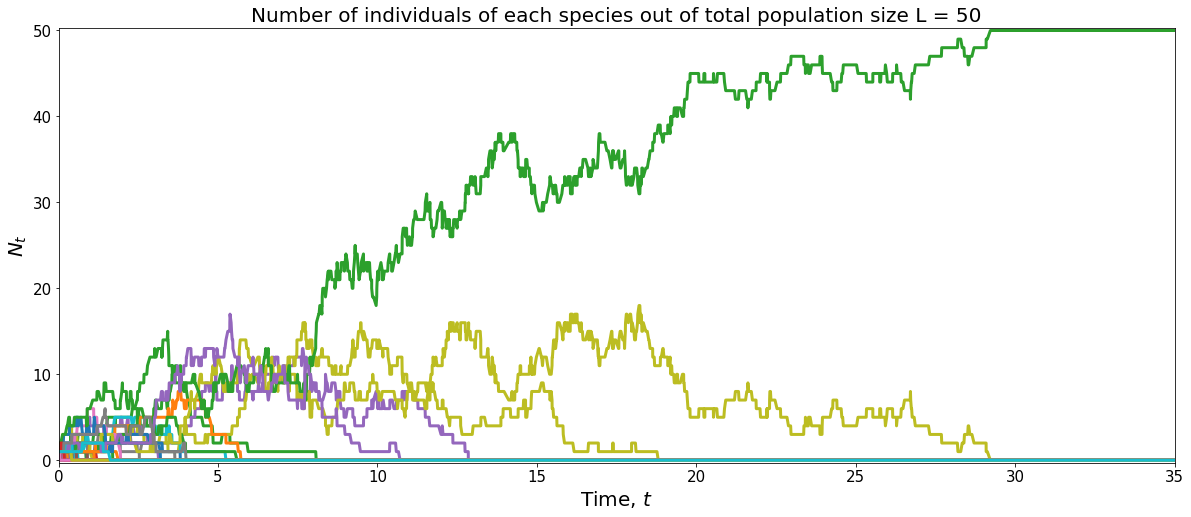
\includegraphics[width = 190mm]{moran}

\end{enumerate}

\section{Barab\'asi-Albert Model}
\begin{enumerate}[a)]
\item
\text{}\\
\hspace*{-2cm}
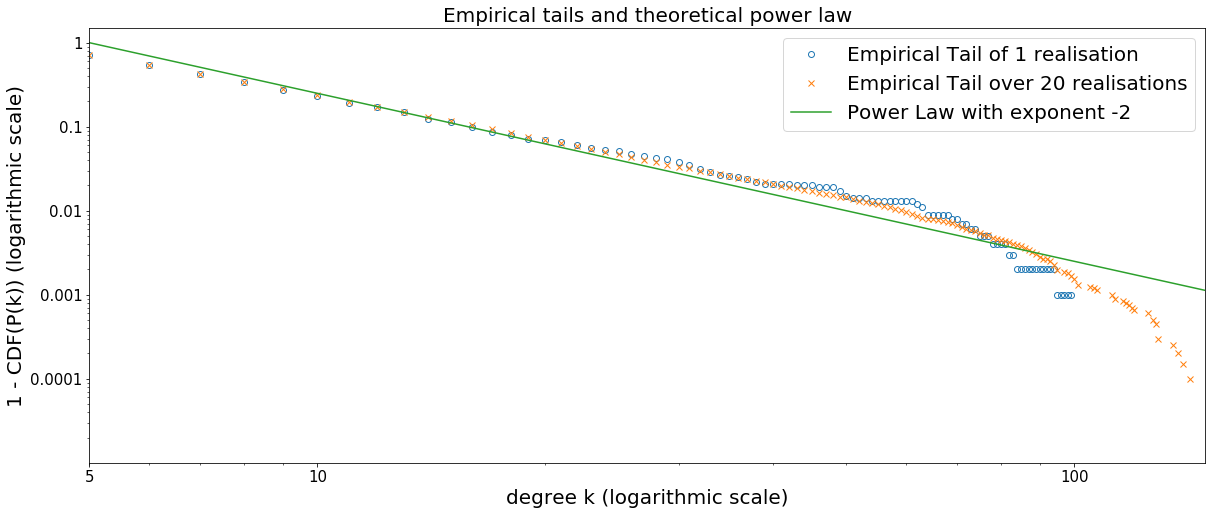
\includegraphics[width = 190mm]{tail}

\vspace{100mm}

\item
\text{}\\
\hspace*{-2cm}
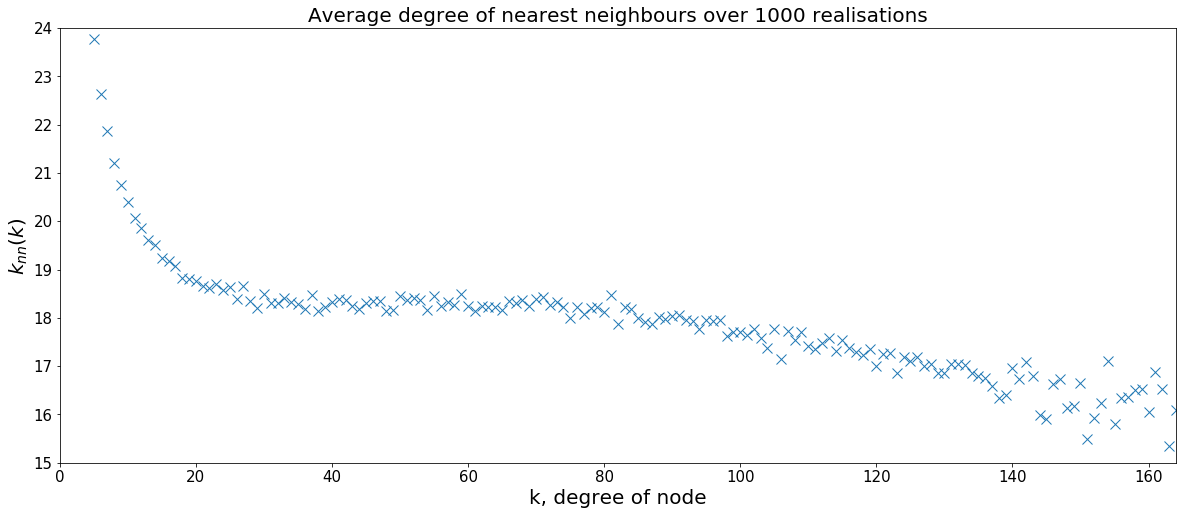
\includegraphics[width = 190mm]{knn}

The plots, and therefore the graphs, appear to be mostly uncorrelated when we only allow 20 realisations of the simulation. There is a very large spread in the data. 

Running the simulation for larger numbers of realisations, $N=1000$ for example, seemed to help smooth out the plot and highlight the disassortative nature of the graphs that we would expect from the theory - I have included that plot below. 

\text{}\\
\hspace*{-2cm}
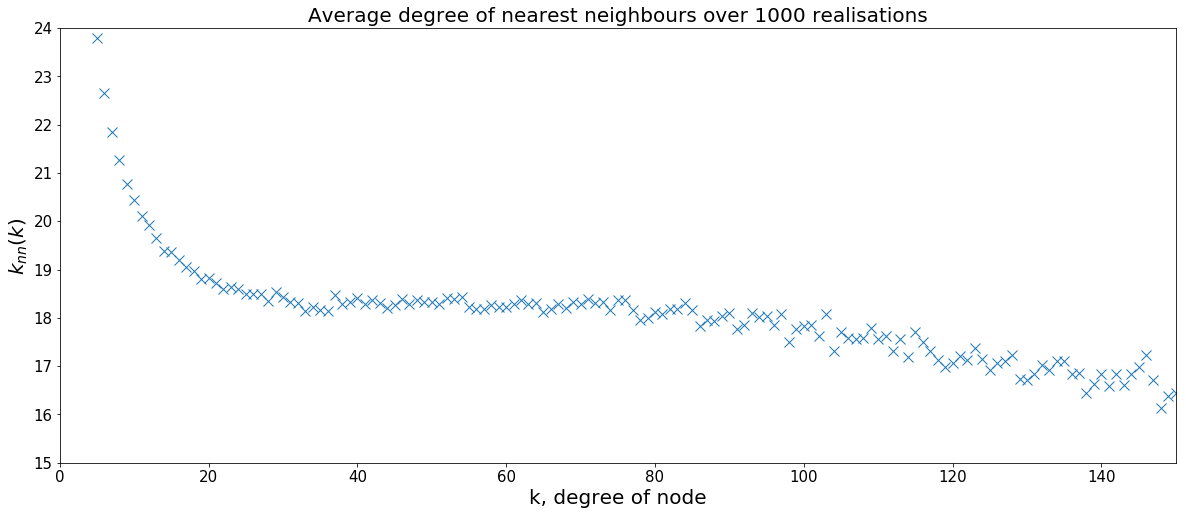
\includegraphics[width = 190mm]{knn1000} 


\end{enumerate}

\section{Erd\"os R\'enyi Random Graphs}
\begin{enumerate}[a)]
\item 
\text{}\\

\begin{figure}[h]
\hspace*{-1.2cm}
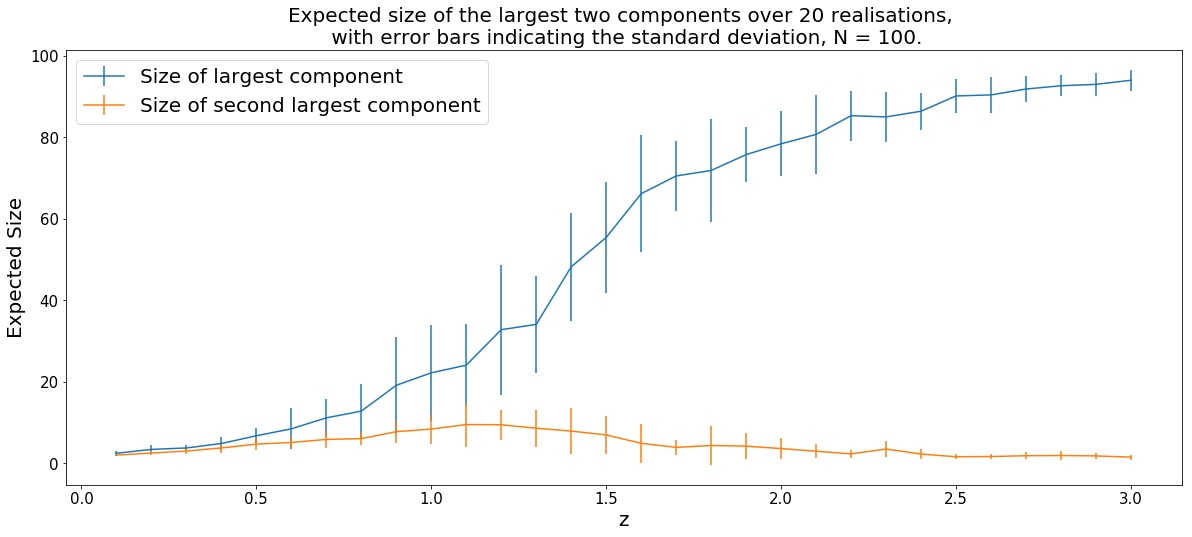
\includegraphics[width = 190mm]{lc100}
\end{figure}


\begin{figure*}[h]
	\hspace*{-1.2cm}
	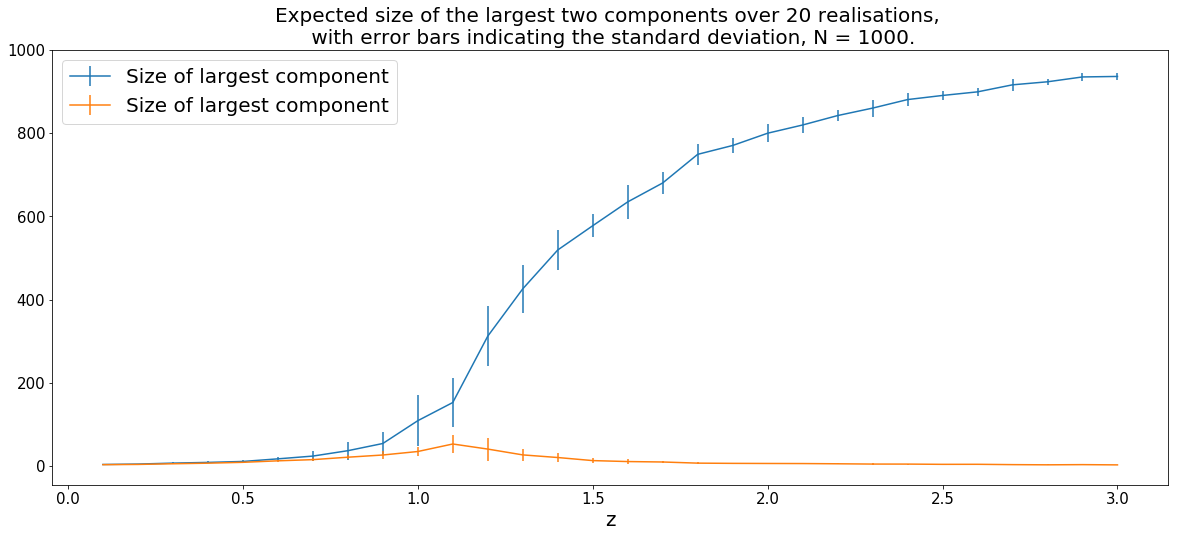
\includegraphics[width = 190mm]{lc1000}
	\end{figure*}

\vspace{100mm}

\item
\text{}\\
\hspace*{-2cm}
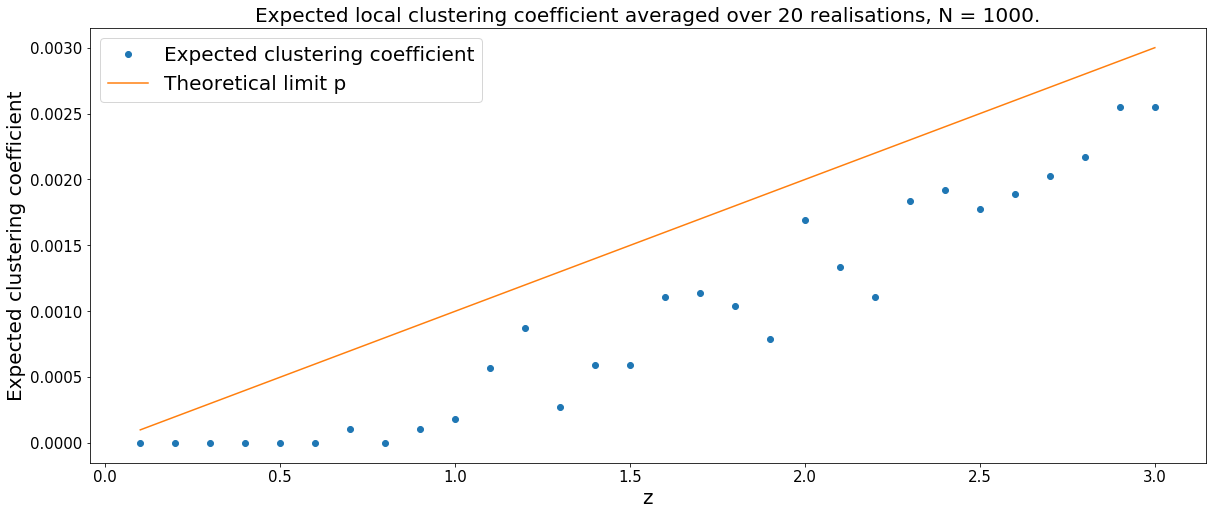
\includegraphics[width = 190mm]{clustering}

The theoretical limit p line fits a lot better when we allow for higher values of $z$. 

%\vspace{100mm}

\item 
\text{}\\
\hspace*{-2cm}
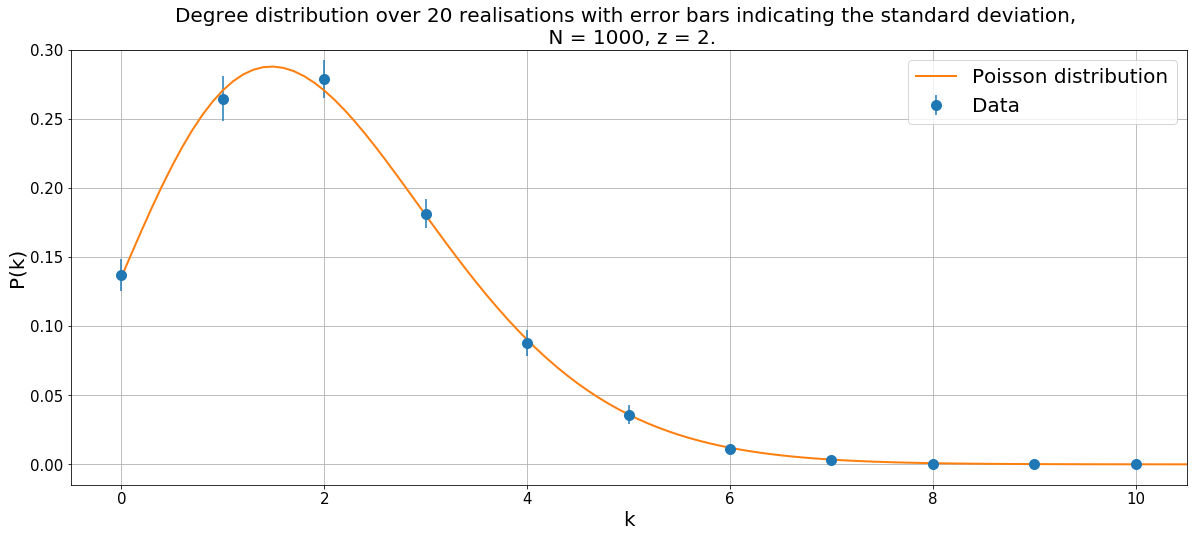
\includegraphics[width = 190mm]{degreedistribution}

I interpreted this question as collate all 20 realisations together to obtain one single degree distribution $p(k)$ but then discovered that some people have plotted all the realisations separately. Therefore I settled and added some error bars. 

\end{enumerate}










\end{document}